\chapter{Architettura del Sistema}
\label{cap:architettura}
\thispagestyle{empty}

\begin{quotation}
{\footnotesize
\noindent \emph{Doc: Questo rende possibile viaggiare nel tempo... il flusso canalizzatore.
Marty: Flusso canalizzatore?! \\
Doc: Mi ci sono voluti quasi 30 anni e tutto il mio patrimonio per realizzare la visione di quel giorno... mio Dio quanto tempo è passato! \\
\dots \\
Marty: Questa... questa è proprio forte Doc! E' grande! Ma funziona con la benzina normale? \\
Doc: Sfortunamente no! Ha bisogno di un qualcosa di un pò più vivace: Plutonio.
}
\begin{flushright}
Ritorno al Futuro, parte I
\end{flushright}
}
\end{quotation}
\vspace{0.5cm}

\section{Introduzione}
In questo capitolo descriveremo l'architettura del sistema, sia dal punto di vista logico, descrivendo la metodologia alla base della soluzione presentata, sia dal punto di vista architetturale, descrivendo nello specifico come è implementato il sistema, come comunicano i moduli implementati e quali tecnologie sono state utilizzate.

Il sistema implementato è pensato per risolvere il problema della localizzazione ad alto livello, cercando di riconoscere oggetti nell'immagine, anziché feature estratte dall'immagine come keypoint, linee o altri tipi di descrittori a basso livello, che possono essere facilmente confusi. Utilizzare oggetti noti nell'immagine, permette di estrarre conoscenza ulteriore sulle caratteristiche spaziali dell'ambiente, infatti le dimensioni dell'oggetto possono essere note, almeno in maniera approssimata. Inoltre il nostro approccio permette di creare mappe semantiche sulle quali è possibile fare inferenza di vario tipo, inferenza che può essere sfruttata anche per migliorare la navigazione stessa.

\section{Architettura Logica}
Per risolvere il problema descritto, abbiamo ritenuto necessario avere i seguenti moduli:

\begin{itemize}
 \item Un reasoner in grado di analizzare di dati e classificare feature.
 \item Un algoritmo di individuazione dei possibili oggetti interessanti.
 \item Un algoritmo di tracking che segua gli oggetti interessanti.
 \item Un algoritmo di riconoscimento degli oggetti individuati come interessanti, cercando di raffinare la classificazione.
 \item Un algoritmo che utilizzi le feature ad alto livello estratte per localizzare il robot nella mappa
\end{itemize}

La struttura logica del sistema implementato è rappresentata in \autoref{fig:locica-sistema}.

\begin{figure}[ht]
  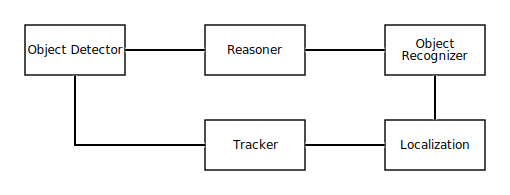
\includegraphics[width=\textwidth]{diagrammi/SchemaLogico}
  \caption{Schema logico del sistema}
  \label{fig:locica-sistema}
\end{figure}

\subsection{Individuazione degli oggetti}
L'individuazione degli oggetti è la base di partenza per l'estrazione dei punti di riferimento su cui si basa la localizzazione.
\`E in grado di analizzare una immagine generica e di estrarre i possibili oggetti significativi. Non è di grande importanza avere un riconoscimento con un alto tasso di recupero, ma è necessario che sia il più preciso possibile, per discriminare le feature interessanti dal rumore.
Non è necessario che il riconoscimento di basso livello sia in grado di distinguere efficacemente le diverse classi di feature cercate, poiché l'analisi approfondita della feature verrà effettuata in altri sottosistemi.
L'individuazione degli oggetti dipende fortemente dal sistema di reasoning.
Questo sottosistema è descritto nel \autoref{cap:riconoscimento}.

\subsection{Reasoner}
Il reasoner è il cuore del sistema, infatti è in grado di analizzare dati rumorosi e incerti e classificare istanze di possibili oggetti trovati dagli algoritmi di estrazione delle feature. Per poter svolgere questo compito in maniera efficace, e per poter affrontare in maniera rigorose le incertezze, si è deciso di utilizzare un reasoner basato sulla logica fuzzy.
Per poter classificare oggetti il reasoner è in grado di ricevere informazione a partire da una knowledgebase, che contiene sia le classi che descrivono gli oggetti, sia le informazioni per interpretare in maniera simbolica i descrittori delle feature, che sono dati numerici. 
Poiché gli oggetti nel mondo reale sono definiti in base alle relazioni con gli altri oggetti, il reasoner è in grado di analizzare queste relazioni per permettere di compiere classificazioni avanzate.
Il reasoner è descritto nel \autoref{cap:reasoning}.

\subsection{Tracker}
Il tracker deve essere in grado di seguire oggetti complessi, che possono uscire dall'immagine o essere parzialmente coperti. Per questo abbiamo implementato il tracker utilizzando un algoritmo di tracking a lungo termine. Grazie a questo tipo di algoritmi non è necessario avere un alto tasso di recupero per il sistema di individuazione degli oggetti, in quanto l'oggetto inseguito viene individuato automaticamente e con un buon tasso di confidenza nell'immagine. Grazie al tracker a lungo termine, possiamo associare con alta confidenza una determinata track a un punto di riferimento nell'algoritmo di localizzazione.
Poiché lo scopo del sistema è di utilizzare la massima informazione possibile in maniera intelligente, l'algoritmo di tracking è in grado di ricevere informazione dalla mappa e processarla per aumentare le sue performance.
L'algoritmo di tracking è descritto nel \autoref{cap:tracking}.


\subsection{Riconoscimento degli oggetti}
Lo scopo di questo sottosistema è quello di implementare un algoritmo di riconoscimento di oggetti ad alto livello. Sfrutta l'informazione proveniente dal tracker per limitare l'analisi di immagine a una regione di interesse il più ristretta possibile, per aumentare le prestazioni sia computazionali sia di riconoscimento. L'informazione estratta da questo nodo può essere utilizzata per etichettare i punti di riferimento nella mappa o per aiutare la localizzazione, fornendo informazioni ulteriori all'algoritmo di localizzazione.
Il riconoscimento degli oggetti è descritto nel \autoref{cap:riconoscimento}.

\subsection{Localizzazione}
La localizzazione è effettuata utilizzando tutta l'informazione estraibile dai sensori e dal resto del sistema.
Il sottosistema che si occupa della localizzazione è in grado quindi di leggere i dati dai sensori del robot e utilizzare i dati estratti dal sistema di riconoscimento delle feature per creare una mappa e cercare di localizzarsi nella maniera più robusta possibile.
Il sistema di localizzazione è pensato per poter utilizzare sia l'informazione proveniente dal tracker, sia l'informazione proveniente dal riconoscimento degli oggetti.
Parleremo della localizzazione nel \autoref{cap:mapping}.

\section{Architettura Software}
Il sistema è stato progettato in maniera modulare per una serie di motivi: questo tipo di architettura permette di riutilizzare i moduli sviluppati, di estendere semplicemente il sistema con altri moduli, di sostituire eventualmente un intero modulo con un altro che compia le stesse funzioni, di comunicare in maniera semplice con altri sistemi. 

Per raggiungere questo scopo, si è deciso quindi di utilizzare il middleware ROS (Robot Operating System)~\cite{quigley2009ros}.
ROS è un middleware che, oltre ad offrire molti strumenti utili per lo sviluppo di complesse applicazioni robotiche, implementa due pattern architetturali importanti, entrambi usati nel nostro lavoro: il pattern publish-subscribe e il pattern client-server.
Questi due pattern sono implementati rispettivamente tramite messaggi e servizi: i messaggi definiscono un formato comune per la pubblicazione di dati in topic, i servizi invece specificano un'interfaccia per le chiamate a procedure remote, dichiarando gli input e gli output tra client e server.

Ogni processo che viene eseguito in ROS è chiamato nodo. Per eseguire qualsiasi sistema basato su ROS, devono essere presenti tre ulteriori nodi: il nodo Master, che si occupa di garantire la comunicazione tra gli altri nodi, tramite i due pattern supportati, il server dei parametri, che implementa un dizionario condiviso accessibile tramite la rete, in cui i nodi possono memorizzare e recuperare parametri usati dai loro algoritmi a runtime, il nodo \textit{rosout}, che si occupa di mantenere i log prodotti dalle applicazioni.

Il sistema sviluppato è pensato per interagire con qualsiasi tipo di robot che sia provvisto di una videocamera monoculare e una unità di misura inerziale (IMU), e eventualmente, un magnetometro, tramite le tre interfacce standard di ROS.
Esse consistono in quattro topic: ``imu'', per i dati provenienti dall'unità di misura inerziale, ``image\_raw'', per l'immagine proveniente dalla videocamera, ``camera\_info'', che contiene i parametri intrinseci della videocamera, tra cui la matrice di calibrazione della videocamera utilizzata, necessaria per il funzionamento del sistema, ``mag'' per i dati provenienti dal magnetometro.
I dati estratti dall'unità di misura inerziale devono poter essere riferiti al sistema di coordinate della videocamera, dato che l'algoritmo di visione implementato utilizza i dati provenienti dalla IMU per stimare approssimativamente la posa della telecamera.
Per rendere l'algoritmo portabile, si utilizza a libreria tf di ROS. La libreria tf gestisce le trasformazioni da un sistema di coordinate all'altro, pubblicando un albero di trasformazioni nel topic ``tf''.
Negli header dei messaggi standard di ROS è definito il campo ``frame\_id'', che descrive il nome del sistema di coordinate rispetto al quale è riferito il contenuto del messaggio. Grazie a questo, è possibile riferire i dati della IMU rispetto alle coordinate dell'immagine, purché sia nota la trasformazione tra i due frame.

\subsection{Diagramma del sistema}

\begin{figure}[ht]
  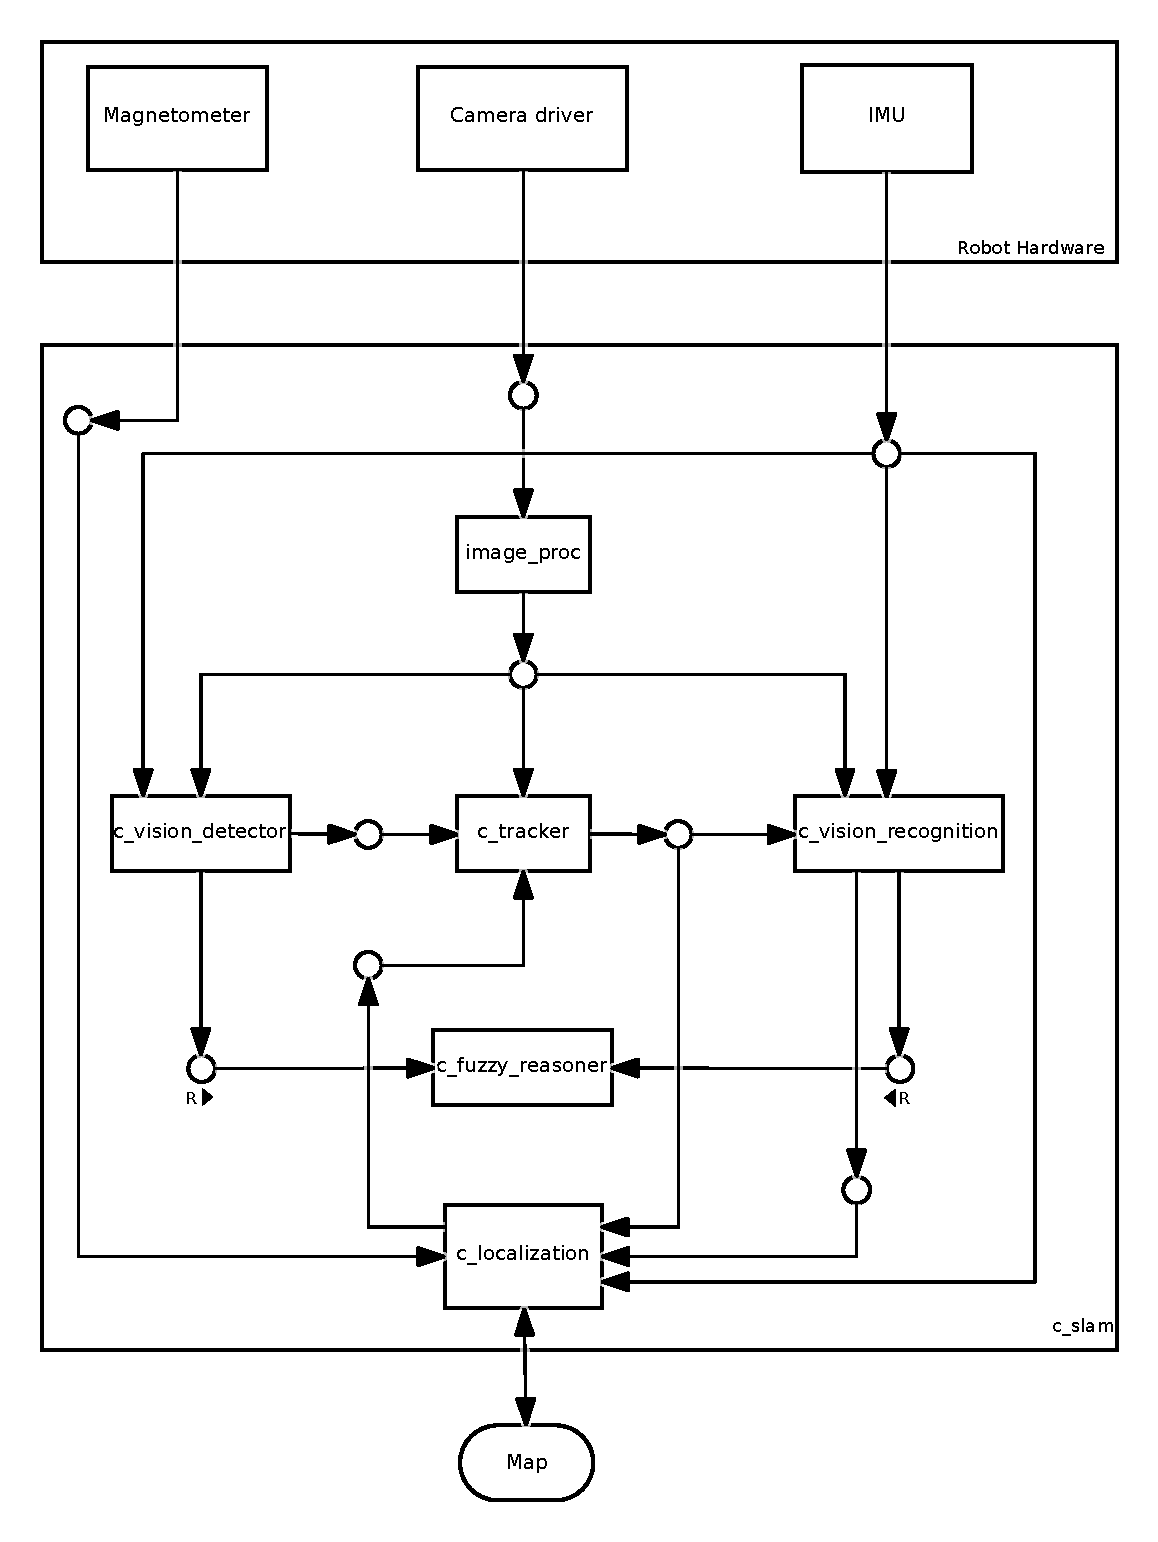
\includegraphics[width=\textwidth]{diagrammi/Sistema}
  \caption{Architettura del sistema implementato}
  \label{fig:architettura-sistema}
\end{figure}

L'architettura del sistema implementato è descritta in \autoref{fig:architettura-sistema}.
Il diagramma rappresenta i nodi del sistema, segue una breve descrizione di ogni elemento per specificare la loro funzione:

\begin{description}
  \item [image\_proc] si occupa di eliminare la distorsione radiale della videocamera causata dalla curvatura della lente.
  \item [c\_vision\_detector] si occupa di estrarre possibili feature dall'immagine.
  \item [c\_tracking] si occupa di seguire le feature a basso livello estratte dal nodo ``c\_vision\_detector'' nell'immagine, mantenendo un modello in modo da riuscire a riconoscere la feature anche dopo essere stata persa. 
  \item [c\_vision\_recognition] si occupa dell'analisi approfondita delle feature, in modo da determinare il tipo di oggetto. 
  \item [c\_fuzzy\_reasoner] implementa un reasoner fuzzy; data una base di conoscenza e un classificatore, analizza le feature in ingresso e le classifica. 
  \item [c\_localization] si occupa di mappare le feature nello spazio e di localizzare il robot nella mappa costruita.
\end{description}

\clearpage


\subsection{Comunicazione tra i nodi}

Il sistema sviluppato sfrutta per la comunicazione tra i nodi sia il paradigma client-server, per l'interazione con il reasoner, sia il paradigma publish-subscribe, in tutti gli altri casi.
Il reasoner offre quattro servizi:

\begin{description}
 \item [\/reasoning] è un  servizio di reasoning basato su una knowledge base fuzzy
 \item [\/classification] si occupa di classificare istanze di feature riconosciute
 \item [\/getDependencyGraph] restituisce il grafo delle dipendenze del classificatore
 \item [\/getReasoningGraph] restituisce il grafo di reasoning utilizzato dal classificatore
\end{description}

Il reasoner e i suoi servizi verranno discussi approfonditamente  nel \autoref{cap:reasoning}.

le informazioni riguardanti gli oggetti riconosciuti e seguiti dal sistema sono scambiate tramite i seguenti topic:

\begin{description}
 \item [\/to\_track] in questo topic vengono pubblicate le possibili feature riconosciute dall'intera immagine. Viene fornito il contorno della feature e la sua possibile classificazione
 \item [\/tracks] in questo topic vengono pubblicati i risultati dell'algoritmo di tracking: contiene il bounding box e il contorno della feature, quest'ultimo viene maggiorato del 20\%, per assicurarsi di mantenere all'interno di esso il reale contorno della feature
 \item [\/visible] in questo topic vengono pubblicate le feature che la localizzazione si aspetta di vedere nella mappa, in modo da agevolare il funzionamento del tracker.
 \item [\/recognized\_objects] in questo topic vengono publicati i risultati del riconoscimento degli oggetti.
\end{description}


\subsection{Parametri degli algoritmi}

Gli algoritmi utilizzati nel sistema, in particolare gli algoritmi di visione, hanno alcuni parametri che è possibile tarare per adattare il sistema a qualsiasi tipo di robot utilizzato.
Per gestire i parametri, abbiamo utilizzato il server dei parametri di ROS.
Il server dei parametri è un dizionario, ossia ogni parametro, identificato da una stringa, è salvato nel server dei parametri, e può essere recuperato tramite il suo nome. 
Il server dei parametri supporta dizionari gerarchici, in modo da poter rappresentare tipi di dati strutturati. 
Inoltre è possibile definire parametri privati per qualsiasi nodo. I parametri privati restano accessibili da tutto il resto del sistema, ma nel dizionario vengono salvati sotto il nome del nodo a cui appartengono; questa caratteristica è fornita per evitare collisioni tra parametri con lo stesso nome in nodi differenti.

Visto che gli algoritmi di estrazione e analisi delle feature si basano fortemente sugli stessi strumenti, il sistema sviluppato usa in maniera estesa i parametri privati, in modo da avere un parametro, che rappresenta concettualmente la stessa quantità, differente per ogni nodo che lo utilizza.

Il sistema permette anche di cambiare i parametri a runtime: essi vengono aggiornati nei nodi che ne fanno uso con una frequenza fissa.
I parametri usati dal sistema e il loro significato sono riportati nell'\autoref{app:manuale}.
